\documentclass[whitelogo]{tudelft-report}

%% Packages
\usepackage{natbib}
\usepackage{changes}
\usepackage{tabu}
\usepackage{booktabs} %for horizontal lines in tables: \toprule[1pt], \midrule[1pt], \bottomrule[1pt]

%% Layout: customized for this certain report
\setlength{\parindent}{0cm} %no indentation in first line of paragraph

%% Compilation: to compile the pdf do (if it is not done automatically):
%% xelatex report
%% bibtex report
%% xelatex report
%% xelatex report


\begin{document}

%% Use Roman numerals for the page numbers of the title pages and table of
%% contents.
\frontmatter

%% Uncomment following 19 lines for a cover with a picture on the lower half only
%\title[tudelft-white]{Title}
%\subtitle[tudelft-cyan]{Optional subtitle}
%\author[tudelft-white]{J.\ Random Author}
%\affiliation{Technische Universiteit Delft}
%\coverimage{cover.jpg}
%\titleoffsetx{10cm}
%\titleoffsety{10cm}
%\afiloffsetx{1cm}
%\afiloffsety{18cm}
%\covertext[tudelft-white]{
%    \textbf{Cover Text} \\
%    possibly \\
%    spanning 
%    multiple 
%    lines
%    \vfill
%    ISBN 000-00-0000-000-0
%}
%\makecover

%% Uncomment following 16 lines for a cover with a picture on the lower half only
\title[tudelft-white]{CIE5308}
\subtitle[tudelft-black]{Breakwater Rehabilitation Romano Port}
\author[tudelft-white]{{J. Gundlach} -- {C. Rozas} -- {L. Lange}}
\affiliation{Delft University of Technology}
\coverimage{title.jpg}
\covertext[tudelft-white]{
    \textbf{Group 3} \\
    %possibly \\
    %spanning 
    %multiple 
    %lines
    \vfill
}
\setpagecolor{tudelft-cyan}
\makecover[split]


%% Include an optional title page.
\input{title}

% \input{preface}

\tableofcontents

%% Use Arabic numerals for the page numbers of the chapters.
\mainmatter

%\input{sections/notes}
\chapter{Introduction}

\section{General Task}

By \textit{Group 3} the breakwater in the South is looked at:
\begin{itemize}
 \item adjacent to roundhead, axis 315\textsuperscript{o}
 \item rubble mound single layer cubes
 \item rehabilitation
 \item 100 years design life
 \item quay wall in future
\end{itemize}

\begin{center}
\begin{table}[!htb]
\begin{tabu}{X[2l] X[1c] X[2c]}
\toprule[2pt]
\textbf{Parameter} & \textbf{Value} & \textbf{Comment}\\
\\
\midrule
Design life                    & 100 years     & \\
Annual downtime                & 3\%           & \\
Quay level                     & AL+2.0m       & \\
Current rock armour (seaward)  & 3 to 5 tons   & \\
Current rock armour (landward) & 0.5 to 3 tons & \\
Current core material          & 0 to 1000 kg  & quarry run material\\

\bottomrule[2pt]
\end{tabu}
\caption{Parameters given by exercise}
\label{tab:paramsExercise}
\end{table}
\end{center}
\chapter{Design Criteria}

see exercise 3.1

\begin{center}
\begin{table}[!htb]
\begin{tabu}{X[2l] X[1c] X[2c] X[1c] X[1c]}
\textbf{Requirement} & \textbf{Return period} & \textbf{Verification method(s)} & \textbf{Design value} & \textbf{Calculated value}\\
\\
\toprule[2pt]
this is supposed to be a verly long text to check whether it will automatically insert a line break & this is supposed to be a verly long text to check whether it will automatically insert a line break & this is supposed to be a verly long text to check whether it will automatically insert a line break & this is supposed to be a verly long text to check whether it will automatically insert a line break & this is supposed to be a verly long text to check whether it will automatically insert a line break\\
\\
× & × & × & × & ×\\
\\
× & × & × & × & ×\\
\\
× & × & × & × & ×\\
\\
× & × & × & × & ×\\
\\
× & × & × & × & ×\\
\\
× & × & × & × & ×\\
\\
× & × & × & × & ×\\
\\
× & × & × & × & ×\\
\\
× & × & × & × & ×\\
\bottomrule[2pt]
\end{tabu}
\caption{List of requirements}
\label{tab:requirements}
\end{table}
\end{center}

\chapter{Boundary Conditions}

see exercise 3.2

\section{Location}

\section{Subsoil}

\section{Reference levels}

\section{Bathymetry}

\section{Waves}
The design storm with less than 20\% probability of failure of the breakwater within a lifetime of 100 years returns every 500 years.
The available 22 years of (modelled) wave data\footnote{ARGOSS XX} close to the site is analysed in a Peak over Threshold analysis using a threshold of $H_s=1.5m$, a storm duration of nine hours and a Weibull distribution to extrapolate the data.
This yields a significant wave height of $H_{ss}=7.91m$ for a 500 year storm, which is chosen to be the deep water design wave height: $H_{ss,d}=7.91m$.


\chapter{Design Calculations}

see exercise 3.3
\chapter{Drawing}

see exercise 3.4


\clearpage
\Huge{This is one single page, where we can add the folded A3 of our drawing after printing.
Included to not interrupt counting of pages.}
\newpage
\chapter{Construction Method and Planning}

\section{Construction Method}

The main steps during construction are:
\begin{enumerate}
 \item Reposition old core
 \item Place core
 \item Place sublayer
 \item Place armour layer on landward side
 \item Place toe
 \item Place armour layer on seaward side
 \item Construct road and top structure
\end{enumerate}

\begin{figure}[!htb]
  \center
  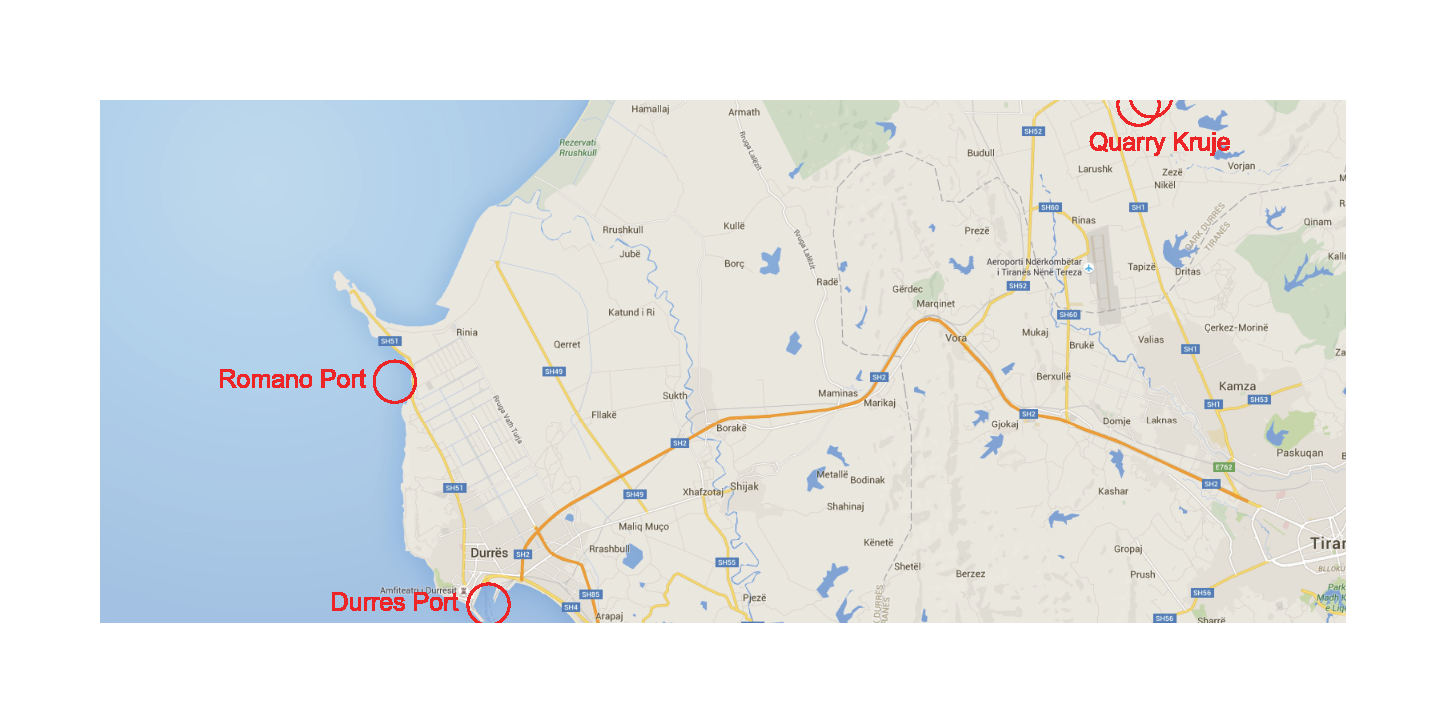
\includegraphics[width=\textwidth]{images/mapConstruction} 
  \caption{Location of facilities needed for construction (map from maps.google.com)}
  \label{fig:mapConstruction}
\end{figure}

\paragraph{Reposition old core}
To increase available space on the side of the harbour the old core is repositioned by moving the armour layer on the harbour side to the seaward side.
The total width of the old breakwater is about 70m at ground level, which poses restrictions on the equipment, that can be used.
Waterborne equipment is not a good choice for this task.
The rocks picked up on the one side (for instance by a hydraulic excavator/crane on a pontoon) would need to be transported to the other side (by a barge for instance), since the hydraulic excavator/ crane would not be able to reach all the way over the old breakwater.
Therefore a landbased long reach hydraulic excavator is used.
For instance Hitachi ZX850 with a reach of 27m and 2m³ bucket capacity could be used\footnote{http://www.land-water.co.uk/group-services/plant-hire-2/long-reach/zx-850-27m-long-reach-excavator/}.
According to \citet{cem} rocks with 0 to 5t have a nominal diameter of maximum 1.38m, thus an average volume of $\frac{4}{3}\Pi \cdot \left(\frac{1.38m}{2}\right)^{3}=1.4m^3<2m^3$, which is smaller than the bucket capacity.
Since the old breakwater is in general expected to be not accessible any more a temporary road will be built buy placing gravel with dump trucks and make them even with a bulldozer (starting from the landside and proceeding to tip of breakwater).
At the end a place to turn around is built.
The width is 8m at least, so two trucks can easily pass each other and a crane or hydraulic excavator at some point does not hinder the truck transport.
For parts of the old breakwater, where the damage is even more severe than depicted in cross-section A-A and B-B a hydraulic excavator/crane on a pontoon will be available to move rocks out of reach of the long reach hydraulic excavator inside its reach.

\paragraph{Place core}
The rocks for the core are delivered from quarry Kruj\"{e}.
There rocks up to 2t are available \citep{MScRomano}.
The distance of about 50km can easily be travelled by trucks (see \ref{fig:mapConstruction}). 
Class 0.3t to 1t is used.
Using the temporary road first on the slopes the needed core material is placed with dump trucks directly coming from the quarry and hydraulic excavators to construct the slope.
This can be done at several positions at one time, depending on the availability of hydraulic excavators and dump trucks.
To reach the lowest points of the breakwater, which might be out of reach, a pontoon with a hydraulic excavator or a crane is available.
Then starting from the tip of the breakwater the needed height of the core will be built.

\paragraph{Place sublayer}
The sublayer is made of rocks of up to 2.5t.
The maximum rocks of 2t available via the quarry are used instead.
They are delivered in a class 1t to 2t.
Same procedure is apllied as for the core, but just in the outer slope.

\paragraph{Place armour layer on landward side}
The armour layer consists of the same rocks as delivered for the sublayer.
The armour layer is placed in the same way as the sublayer, but on the inner slope oof the breakwater.

\paragraph{Place toe}
To hinder erosion at the toe of the structure the same material as delivered for the sublayer and armour layer on the landward side is used to place a toe in front of the breakwater.
Side stone dumping vessels are used to put the toe in place, since it is certainly out of reach and dumping the stones is faster than placing them from a pontoon.
The rocks will be transported to Durres Port by truck across a distance of about 50km.
Use is made of the dry bulk facilities there to load the side stone dumping vessel, which then travels about 15km northwards to the construction side.
There it dumps the stones and returns to be loaded again.


To show how the different steps given above interlock with each other see \nameref{chap:appendixB}.

\section{Production Calculation}
\chapter{Further Research and Validation}

see exercise 3.6


%% Use letters for the chapter numbers of the appendices.
\appendix

\chapter{Appendix A}

 \subsection{Wave-data check}
 
Estimation of fetch-limited Waves; Method of Verhagen and Young: \\
$ \tilde{H}=\tilde{H}_{\infty}[tanh(k_1 \tilde{F}^{m_1})]^p $ with $ \tilde{F}= \frac{g F}{U_{10}^2} $ and $H_{m0} = \frac{\tilde{H} U_{10}^2}{g} $ \\
The input:
\begin{itemize}
\item $\tilde{H}_{\infty}= 0.24 $
\item $k_1= 4.41*10^{-4} $
\item $ m_1= 0.79 $
\item $p= 0.572 $
\item $F= 1000 km $
\item $U_{10}= 20 \frac{m}{s} $
\end{itemize}
 and the results:
 \begin{itemize}
 \item $\tilde{F}=25000 $
 \item $\tilde{H}= 0.22 $
 \item $H_{m0}= 8.8 m $
 \end{itemize}
 8.8 m is the maximum possible wave hight according to the fetch length and the Young/Verhagen method of dimensionless fetch.
 \\
\begin{figure}[H]
\center
\fbox{
 \includegraphics[width=\textwidth]{images/wave_pperiod_allyear.png} 
}
\caption[Distribution of peak-period over wave hight]{Distribution of peak-period over wave hight}
 %\label{Distribution_pperiod}
\end{figure}
% 
% 
\begin{figure}[H]
\center
\fbox{
\includegraphics[width=\textwidth]{images/Rose_plot_u10.png} 
}
\caption{Rose-diagram with the distribution of the wind}
 %\label{Windrose}
\end{figure}
% 
% 
\begin{figure}[H]
\center
\fbox{
\includegraphics[width=\textwidth]{images/Rose_plot_Hoverall.png} 
}
\caption{Rose-diagram with the distribution of the waves}
% %\label{wavedata_angle}
\end{figure}

Whatever XX

\chapter{Appendix B}\label{chap:appendixB}


XX include clip 

\bibliography{report}

\end{document}

